\documentclass[twoside]{article}


%\usepackage{hyperref}
\usepackage{amssymb,amsthm}
\usepackage{amsmath}
\usepackage{color}
\usepackage{ esint }
\usepackage{mathabx}
\usepackage{MnSymbol}
\usepackage{fancyhdr}
\usepackage{soul} 
%\usepackage{times}

%\usepackage[latin1]{inputenc}

\usepackage{comment}
\usepackage{url}
\usepackage{xcolor}
\usepackage{adjustbox}
\usepackage{hyperref}

\newtheorem{thm}{Theorem}[section]
\newtheorem{cor}[thm]{Corollary}
\newtheorem{lem}[thm]{Lemma}

\newtheorem{defi}[thm]{Definition}
\newtheorem{prop}[thm]{Proposition}
\theoremstyle{remark}
\newtheorem{comentario}{Remark}


\makeatletter
\newcommand{\labitem}[2]{%
\def\@itemlabel{\textbf{#1}}
\item
\def\@currentlabel{#1}\label{#2}}
\makeatother




\title{Periodic solutions for a Sitnikov restricted $n+1$-body problem with primaries in rigid motion}
\author{Gast\'on Beltritti \thanks{SECyT-UNRC and CONICET}\\
Dpto. de Matem\'atica, Facultad de Ciencias Exactas Físico-Químicas y Naturales\\
Universidad Nacional de R\'{i}o Cuarto\
(5800) R\'{\i}o Cuarto, C\'ordoba, Argentina,\\
\url{gbeltritti@exa.unrc.edu.ar}\\[3mm]
Fernando D. Mazzone \thanks{SECyT-UNRC, FCEyN-UNLPam}\\
Dpto. de Matem\'atica, Facultad de Ciencias Exactas, F\'{\i}sico-Qu\'{\i}micas y Naturales\\
Universidad Nacional de R\'{i}o Cuarto\\
(5800) R\'{\i}o Cuarto, C\'ordoba, Argentina,\\
\url{fmazzone@exa.unrc.edu.ar}\\
Martina G. Oviedo \thanks{SECyT-UNRC, CIN}\\
Dpto. de Matem\'atica, Facultad de Ciencias Exactas, F\'{\i}sico-Qu\'{\i}micas y Naturales\\
Universidad Nacional de R\'{i}o Cuarto\\
(5800) R\'{\i}o Cuarto, C\'ordoba, Argentina,\\
\url{martinagoviedo@gmail.com}
}

\date{}


\newcommand{\rr}{\mathbb{R}}
\newcommand{\nn}{\mathbb{N}}


\newcounter{example}

\setcounter{example}{1}


\newenvironment{example}{\noindent\textit{Example} \arabic{example}.}{\addtocounter{example}{1}}




\begin{document}


\maketitle
%
% \begingroup%Locallizing the change to `thefootnote'.
%     \renewcommand{\thefootnote}{}%Removing the footnote symbol.
%     %
%     \footnotetext{%
%     %   2010 Mathematics Subject Classification
%     %   http://www.ams.org/msc/
%     \textbf{2010  AMS Subject Classification.} Primary: .
%     Secondary: .
%     }%
%         \footnotetext{%
%     \textbf{Keywords and phrases.}  .
%     }%
%     \endgroup
%
%
%
%

\begin{abstract}


\end{abstract}




\pagestyle{fancy} \headheight 35pt \fancyhead{} \fancyfoot{}

\fancyfoot[C]{\thepage} \fancyhead[CE]{\nouppercase{G. Beltritti, F. Mazzone, M. Oviedo}} \fancyhead[CO]{\nouppercase{\section}}

\fancyhead[CO]{\nouppercase{\leftmark}}


%\tableofcontents




\section{Introduction}
In this paper we study the following restricted  Newtonian $n+1$-body problem $P$ (see figure \ref{fig:conf_esp}):
\begin{itemize}
 \item[$P_1$] We have $n$ primary bodies of masses $m_1,\ldots,m_n$ and an additional massless body.
 \item[$P_2$] The primary bodies are in a central  configuration rigid motion (see \cite[Section 2.9]{JaumeLlibre276}). This motion is periodic and it is carried out in a plane $\Pi$.
 \item[$P_3$] The massless particle is moving  on the perpendicular line to $\Pi$ passing through the center of masses.
\end{itemize}


\begin{figure}[h]
 \begin{center}


\setlength{\unitlength}{4cm}
\begin{picture}(2.5, 1)(-.5, -.5)
  \setlength{\unitlength}{2cm}
    \put(.5,0){
}
  \setlength{\unitlength}{5cm}
    \put(-.1,0){
    \qbezier(0, 0)(0,.25)(.5, .25)
  \qbezier(1.01, 0)(1.01,.25)(.5, .25)
    \qbezier(0, 0)(0,-.25)(.5, -.25)
  \qbezier(1.01, 0)(1.01,-.25)(.5, -.25)
}
\put(-.2,0){\line(1,0){1.2}}
\put(-0.1,0){\circle*{.04}} \put(-0.19,-0.05){$m_1$}
\put(0.65,-0.24){\circle*{.04}} \put(0.61,-0.2){$m_2$}
\put(0.6,.235){\circle*{.04}}\put(0.55,.18){$m_3$}
\put(0.5,0){\circle*{.03}}\put(0.44,-0.05){$c$}
\put(0.5,-0.08){\line(0,1){.6}}
\put(0.5,0.4){\circle*{.04}}\put(0.53,0.4){$m_4\approx 0$}
\put(-.3,-0.3){\line(1,0){1.5}}
\put(-.3,-0.3){\line(1,5){.12}}
\put(1.2,-0.3){\line(-1,5){.12}}
\put(-0.18,0.3){\line(1,0){1.26}}
\put(1.1,-0.25){$\Pi$}
\end{picture}\caption{Four-body problem with three primaries}\label{fig:conf_esp}
 \end{center}

\end{figure}

Problems like the one presented have been extensively discussed in the literature. In \cite{sitnikov1960existence} K. Sitnikov considered the problem of two body in a Keplerian motion and a massless particle moving in the perpendicular line to the orbital plane passing
through the center of masses. Sitnikov obtained deep results about existence of solutions, some of them periodic (see \cite[III(5)]{moser2016stable}). Since then many  other authors have studied Sitnikov problem, for instance  Liu, Zhou, and Sun \cite{liu1991numerical},  Hagel and Trenkler \cite{hagel1993computer}, Dvorak \cite{dvorak1993numerical}, Dankowicz and Holmes \cite{dankowicz1995existence}, Llibre, Meyer and Soler \cite{llibre1999bridges}, Chesley \cite{chesley1999global}, Jim{\'e}nez-Lara a and Escalona-Buend{\'\i}a \cite{jimenez2001symmetries},
 Llibre and Ortega \cite{llibre2008families}, P{\'e}rez, Jim{\'e}nez and Lacomba \cite{perez2009periodic}.

Problems like the Sitnikov problem for four bodies  were addressed more recently.
In \cite{soulis2008periodic} Soulis, Papadakis and Bountis studied existence, linear stability and bifurcations for a problem similar to $P$. They considered  a Lagrangian equilateral triangle configuration for the primaries bodies, which were supposed to have the same mass $m_1=m_2=m_3$. In \cite{bountis2009stability} Papadakis and Bountis extend of results of \cite{soulis2008periodic} to $N-1$ primaries ($N\geq 4$) in a poligonal equal mass configuration. Later  in \cite{pandey2013periodic}, Pandey and Ahmad extend the analysis started in \cite{soulis2008periodic} to the case when the primaries are oblate (not mass points).
In \cite{zhao2015nonplanar}, Zhao and Zhang proved existence, by means of a variational approach, of periodic solutions for a problem similar to the one dealt in \cite{soulis2008periodic}.
In \cite{li2013characterization} Li, Zhang and Zhao studied a special type of
restricted circular $N+1$-body problem  with equal masses for the primaries in a regular polygon configuration.

In the present paper we extend the analysis in \cite{zhao2015nonplanar} to the case of a collinear central configuration for the primaries.





\section{Preliminaries and Main Results}

We start considering $n$  mass points, $n>2$, of masses $m_1,\ldots,m_n$ moving in a Euclidean 3-dimensional space according to Newton's laws of motion. We assume that $q_1(t),\ldots,q_n(t)$ are the coordinates (column vectors) of the bodies in some inertial Cartesian coordinate system. We denote by $r_{ij}=|q_i-q_j|$  the  Euclidean distance between $q_i$ and $q_j$. We can suppose, without any loos generality, that the center of mass   $c:=\sum_jm_jq_j/M$ ($M:=\sum_j m_j$) is fixed at the origin ($c=0$).

We assume that these bodies are in a \emph{rigid motion}. We recall that a \emph{rigid  motion}, is a solution of motions equations with $r_{ij}$ constant.  It is known (see \cite{ AurelWintner272}) that a rigid motion is performed in a plane $\Pi$. We assume that $\Pi$ is the plane determined by the first two coordinates axes. Then a rigid motion has the form (see \cite{JaumeLlibre276})
\[q_j(t)=Q(\nu t)q^0_j,\]
where
\[
 Q(\nu t)=\begin{pmatrix}
           \cos(\nu t) & -\sin(\nu t) & 0\\
           \sin(\nu t) & \cos(\nu t) & 0\\
           0            &     0     &  1\\
          \end{pmatrix}
\]
and $q^0_j\in\Pi$, $j=1,\ldots,n$ are vectors in a planar \emph{central configuration} (CC) in $\rr^3$, i.e. there exists $\lambda\in\rr$ such that
\[ \nabla_jU(q^0_1,\ldots,q^0_n)+\lambda m_jq^0_j=0,\quad j=1,\ldots,n.\]
where the \emph{potential function} $U$ is defined by:
\begin{equation}\label{eq:potencial}
 U(x)=\sum_{i<j}\frac{m_im_j}{r_{ij}},
\end{equation}
and $\nabla_j$ denotes the $3$-dimensional partial gradient with respect to $q_j$.
According to \cite[Eq. (2.16)]{JaumeLlibre276} we have $\nu^2=\lambda$. Then the primaries bodies perform a periodic motion with period $T:=2\pi/\nu$ .

We suppose that we have a massless particle with coordinates $q(t)=(x(t),y(t),z(t))\in\rr^3$. This particle does not disturb the rigid motion of  primaries.  We want to find conditions under which this particle perform a $T$-periodic motion on the $z$ axis of coordinates.

The particle $q$ satisfies the Newtonian equations of motion
\begin{equation}\label{eq:newton}
 \ddot{q}=\sum_{i=1}^n\frac{m_i(q_i-q)}{|q_i-q|^3},
\end{equation}

A necessary and sufficient condition for the particle  has a non-trivial motion along the $z$ axis at all times is that the horizontal component of the gravitational force originated by the primaries is null. The following theorem characterize the initial configuration $(q_1^0,\ldots,q_n^0)$ with this property.


\begin{thm}\label{thm:prim} There exists a non-stationary  solution of \eqref{eq:newton} with $x(t)=y(t)=0$ if and only if $q^0_1,\ldots,q^ 0_n$ satisfy that for any $r>0$, such that the set
\[F_r:=\{i:|q_i^ 0|=r\}\]
is non empty, that
\begin{equation}\label{eq:suma0}\sum_{i\in F_r}m_iq_i^ 0=0.\end{equation}
i.e. every maximal set of  bodies which are equidistant from origin has center of mass equal to $0$.
\end{thm}
We will show by means of an example that non-stationary assumption is necessary.

If condition \eqref{eq:suma0} holds then equation \eqref{eq:newton} is reduced to
\begin{equation}\label{eq:eq_new_red}
 \ddot{z}=-\sum_{i=1 }^n\frac{m_iz}{(s_i^2+z^2)^{\frac32}},
\end{equation}
with  $s_i=|q_i^0|$.




We note that in order to get collisionless solutions of problem $P$ we need that no primary body is located in the center of mass. We say that a
CC is \emph{admissible} if it is non-collisional and satisfies \eqref{eq:suma0}. In the following theorem we characterize all admisible configurations with 3 or 4 bodies.

\begin{thm}\label{thm:caracterizacion}
The only 3-body admissible CC is the equilateral triangle with three equal masses. In the case of 4-body, an admissible CC  has two pairs of equal masses and satisfies some of the following properties: it is collinear and symmetric around the center of mass or it is a rhombus with the equal masses in opposite vertices, being the minor masses near from origin. In the particular case that the four masses  lie in a common circle with center of mass at the origin the CC is a  equal mass square.
\end{thm}

If the equation \eqref{eq:eq_new_red} has a $kT$-periodic solution, where $T$ is the period for the primaries and $k$ is a positive integer, we say that the solution is  $kT$-synchronous.

The following theorem characterize all the possible period for the massless particle.

\begin{thm}\label{thm:prin_ine} We assume that $q_1^0,\ldots,q_n^0$ is a admisible CC.
\begin{enumerate}
 \item\label{1} A non-trivial solution of the equation \eqref{eq:eq_new_red} is either periodic or  its norm tends to infinity when $t$ goes to infinity. The escape velocity for initial condition $z(0)$ is

 \begin{equation}\label{eq:vel.esc}
 V_{Esc}=\left(\sum_{i=1}^{n}\frac{2m_i}{\sqrt{s_i^2+z(0)^2}}\right)^{\frac12}.
 \end{equation}

 \item\label{2} A necessary and sufficient condition for that equation \eqref{eq:eq_new_red} has non trivial $T_0$-periodic solutions is that
\begin{equation}\label{eq:ine_T0-per-cond}
 \frac{4\pi^2}{T_0^2}<\sum_{i=1}^n\frac{m_i}{s_i^3}
\end{equation}
\item\label{3} In particular, there is a $T$-synchronous solution if and only if

\begin{equation}\label{eq:ine_prin}
 \sum_{i<j}\frac{m_im_j}{r_{ij}}<\left(\sum_{i=1}^n\frac{m_i}{s_i^3}\right)\left(\sum_{i=1}^nm_is_i^2\right).
\end{equation}
\end{enumerate}

\end{thm}

We observe that for all admissible CC there exists $kT$ synchronous solution (and therefore a periodic solution of the complete $n+1$-problem) when $k\in \mathbb{N}$ is  large enough.

The sufficiency of the condition $n\leq 472$ in the following corollary  was proved in \cite{li2013characterization}.

\begin{cor}\label{cor:nleq472}
We suppose that $q_1^0,\ldots,q_n^0$ is the equal masses regular polygon configuration  (this is an admisible CC). Then there exists a synchronous solution if and only if $2\leq n\leq 472$.
\end{cor}




Our next objective is to verify that condition \eqref{eq:ine_prin} is satisfied for all admissible CC of 3-body or 4-body. In virtue of Corollary \ref{cor:nleq472} and Theorem \ref{thm:caracterizacion}  we rest prove that condition \eqref{eq:ine_prin} is satisfied for the symmetric collinear $4$-body CC, and for the CC forming a rhombus with equal masses in opposite vertices. Let's call these central configurations CCcl and CCr respectively.



\begin{thm}\label{thm:CC.3.4.satis.cond.adm}
The central configurations CCcl and CCr satisfy condition \eqref{eq:ine_prin}.
\end{thm}

\begin{cor}
For all  admissible CC of 3-body or 4-body  problem $P$ has a $T$-synchronous solution.
\end{cor}




\section{Proofs}



\begin{lem}\label{lem:1} For $c>0$ we define the function $y_c(t):=(c+t)^{-3/2}$. If $0<t_1<t_2<\ldots<t_k$ then the functions $y_j(t):=y_{t_j}(t)$  are linearly independent on  each open interval   $\mathcal{I}\subset \mathbb{R}^+$.
\end{lem}
\begin{proof} It is sufficient to prove that Wronskian

 \[W:=W(y_1,\ldots,y_k)(t)=\det\begin{pmatrix}
			      y_1 & \cdots & y_k\\
			      \frac{dy_1}{dt}&  \cdots & \frac{dy_k}{dt}\\
			      \vdots & \ddots & \vdots \\
			      \frac{d^{k-1}y_1}{dt^{k-1}}&  \cdots & \frac{d^{k-1}y_k}{dt^{k-1}}\\
                           \end{pmatrix}
\]
is not null on $\mathcal{I}$.

Using induction is easy to show that
\begin{equation}\label{eq:der_ind}\frac{d^iy_c}{dt^i}=\beta_{i}y_{c}^{\frac{2i+3}{3}},\quad\hbox{for some }\beta_{i}\neq 0, \hbox{ and for all }i=1,\ldots.
\end{equation}
Fix any $t\in I$. Then, according to \eqref{eq:der_ind} and writing $\lambda_j:=(t+t_j)^{-1}$, we have

\[
\begin{split}
  W(t)&=\det
    \begin{pmatrix}
      \lambda_1^{3/2} & \lambda_2^{3/2} &\cdots & \lambda_k^{3/2} \\
      \beta_1\lambda_1^{5/2} &\beta_1 \lambda_2^{5/2} &\cdots &\beta_1 \lambda_k^{5/2}\\
      \vdots & \vdots &\ddots & \vdots\\
      \beta_{k-1}\lambda_1^{k+1/2} & \beta_{k-1}\lambda_2^{k+1/2} &\cdots & \beta_{k-1}\lambda_k^{k+1/2}
    \end{pmatrix}
  \\
  &= \beta_1\beta_2\cdots\beta_{k-1} \lambda_1^{3/2}\lambda_2^{3/2}\cdots \lambda_k^{3/2}
     \det \begin{pmatrix}
      1& 1 &\cdots & 1 \\
      \lambda_1 & \lambda_2 &\cdots & \lambda_k\\
      \vdots & \vdots &\ddots & \vdots\\
      \lambda_1^{k-1} & \lambda_2^{k-1} &\cdots & \lambda_k^{k-1}
    \end{pmatrix}
  \\
  &= \beta_1\beta_2\cdots\beta_{k-1} \lambda_1^{3/2}\lambda_2^{3/2}\cdots \lambda_k^{3/2}
  \prod_{1\leq i<j\leq n}(\lambda_j-\lambda_i)
,
\end{split}
\]
where the last equality follows of the well known Vandermonde determinant identity. Therefore $W\neq 0$ if and only if $\lambda_i\neq\lambda_j$, $i\neq j$,
which in turn is equivalent to $t_i\neq t_j$, $i\neq j$.
\end{proof}


\begin{proof} [Proof Theorem \ref{thm:prim}] We use a rotating coordinate system where the primaries are fixed. Concretely we  put
\[\xi=Q(-\nu t)q.\]
In this system the motion equations are
\begin{equation}\label{eq:mov_rot}\ddot{\xi}+2\nu B\dot{\xi}+\nu^2 C\xi=\sum_{i=1}^n\frac{m_i(q_i^0-\xi)}{|q_i^0-\xi|^3},\end{equation}
where
\[B:=\begin{pmatrix}
       J & 0_{2\times 1}\\
       0_{1\times 2} & 0\\
     \end{pmatrix},\quad J:=\begin{pmatrix}
       0 & -1\\
       1 & 0\\
     \end{pmatrix}\quad\hbox{and}\quad C=\begin{pmatrix}
       -I_{2} & 0_{2\times 1}\\
       0_{1\times 2} & 0\\
     \end{pmatrix},
\]
where $0_{n\times m}$ and $\mathcal{I}_{n}$ denote the null $n\times m$ matrix  and the identity $n\times n$ matrix respectively. Assuming that the masless particle is moving on the $z$-axis then $\xi=q=(0,0,z)$ and the Coriolis and centrifugal forces,   $2\nu B\dot{\xi}$ and $\nu^2 C\xi$ respectively, are null. Therefore, taking account in the first two equation in \eqref{eq:mov_rot} and identifying the vectors $q_i^0$, $i=1,\ldots,n$ with vectors in $\rr^2$, we have
\[
\sum_{i=1}^n\frac{m_iq_i^0}{|q_i^0-\xi|^3}=0.
\]

Let $D=\{|q_i^0|: i=1,\ldots,n\}$.  Suppose that $D=\{r_1,\ldots,r_k\}$, with $r_i\neq r_j$ for $i\neq j$, and  $\{1,\ldots,n\}=F_1\cup \cdots\cup F_k$, where if $i\in F_j$ then $|q_i^0|=r_j$. Then
\[\sum_{j=1}^k\left\{\frac{1}{(r_j^{2}+z^2)^{3/2}}\sum_{i\in F_j}m_iq_i^0\right\}=0.\]

Since we are considering a non-stationary solution, we have that $z(t)$ is not constant. Therefore there exists an interval $\mathcal{I}\subset\rr^+$ where
\[\sum_{j=1}^k\left\{\frac{1}{(r_j^{2}+s)^{3/2}}\sum_{i\in F_j}m_iq_i^0\right\}=0,\quad s\in I.\]
Then, according to Lemma \ref{lem:1}, we obtain \eqref{eq:suma0}.

If  \eqref{eq:suma0} is satisfied then the force field $F$ acting on the masless
particle carries the $z$ axis in itself. Therefore, from the existence and uniqueness theorem and other elementary properties of system of ODEs we obtain a solution  of \eqref{eq:newton} with $x(t)=y(t)=0$.  \end{proof}


\begin{proof}[Proof Proposition \ref{prop:CCno.adm.sol.trivial}]
Some of the following calculations were made with symbolic math software. Let's  consider a particular Euler's linear central configuration formed by three collinear bodies of mass $m_1 = 4-\mu$, $m_2 = 2 + \mu$, $m_3 = 1$, where $0<\mu<1$, and $q_1 = 0$, $q_2 = 1$ and $q_3 = 1 + r$ their respective positions, with $r$ such that
\[ p(r,\mu)=0,\]
where $p(r,\mu)=6 r^{5} +\left(- \mu + 16\right) r^{4}  +  \left(- 2 \mu + 14\right) r^{3}+ \left(- \mu - 5\right)  r^{2}+\left(- 2 \mu - 7\right) r - \mu - 3$. Note that as $p(0,\mu)=-\mu-3$ and $P(1,\mu)=-7\mu+21$ then, for all $0<\mu<1$, $r\in (0,1)$ .
In this case the center of mass $C$ is equal to $\frac{\mu}{7} + \frac{r}{7} + \frac{3}{7}$, so $C\in (0,1)$. 

We denote with $x$ the point between 0 and 1 where the sum of the forces that the primary bodies make on a massless particle located in that position is equal to zero. For this value of $x$ we have to
$f(x)=0,$ where $f(x)= - \frac{4-\mu }{x^{2}}+\frac{\mu + 2}{\left(- x + 1\right)^{2}} + \frac{1}{\left(r - x + 1\right)^{2}}$.
Note that the left side of the previous equation is an increasing function that tends to $-\infty$ when $x$ goes to 0, and tends to $+\infty$ when $x$ goes to 1, so there is a unique point $x\in (0,1)$, such that the equality holds.

Then, if we want to have a trivial solution of the problem \eqref{eq:newton} then necessarily $C$ has to be equal to $x$. Let's see that there exists $ \mu \in (0,1) $ such that $ C = x $, i.e. $f(C)=0$. For this purpose, since $C$ is a continuous function with respect to $\mu$,  we need to see that there exists a value $\mu_1\in (0,1)$ such that $f (C) <0$  and   $ \mu_2\in (0,1) $ such that $ f (C)> 0 $.  The function $f(x)$ can be factorized as $$f(x)=\frac{Nf(x)}{Df(x)},$$ where $Nf(x)=2 \mu r^{2} x^{2} - 2 \mu r^{2} x + \mu r^{2} - 4 \mu r x^{3} + 8 \mu r x^{2} - 6 \mu r x + 2 \mu r + 2 \mu x^{4} - 6 \mu x^{3} + 7 \mu x^{2} - 4 \mu x + \mu - 2 r^{2} x^{2} + 8 r^{2} x - 4 r^{2} + 4 r x^{3} - 20 r x^{2} + 24 r x - 8 r - x^{4} + 10 x^{3} - 21 x^{2} + 16 x - 4$ and $Df(x)=x^{2} \left(x - 1\right)^{2} \left(r - x + 1\right)^{2}$. Note that  $Df(x)>0$ for all $x\in (0,1)$. If we consider $\mu=0$ and compute $Nf(C)$ we have that
\[Nf(C)=\frac{r^{4}}{2401} + \frac{1514 r^{3}}{2401} + \frac{2245 r^{2}}{2401} + \frac{1110 r}{2401} + \frac{333}{2401}>0,\]
on the other, hand if  $\mu=1$ then
\[Nf(C)=- \frac{71 r^{4}}{2401} + \frac{1486 r^{3}}{2401} + \frac{401 r^{2}}{2401} - \frac{1480 r}{2401} - \frac{592}{2401}<0,\]
because $0<r<1$. 
\end{proof}

\begin{proof}[Proof Theorem \ref{thm:caracterizacion}]
For the case of 3-bodies, we note that the Theorem \ref{thm:prim} and the fact that the center of masses is an excluded position imply that if $F_r$ is not empty then $\# F_r\geq 2$. Hence an admissible 3-body CC consists of three equidistant bodies from the origin. Therefore, it must to be the Lagrangian equilateral triangle configuration. Now, equation \eqref{eq:suma0} implies that every bodies has the same mass.

In the case of 4-bodies, we have again that $\# F_r\geq 2$.  We consider two cases, the first one  $|q_1|\neq|q_2|$.  Therefore we can suppose that $|q_1|=|q_3|$ and $|q_2|=|q_4|$. Now \eqref{eq:suma0} implies that
 $m_1=m_3$ and $m_2=m_4$.  We divide the plane in two cones by means of  the line $L$ joining $q_1$  and $q_3=-q_1$ together with its perpendicular bisector $M$.  From the Perpendicular Bisector Theorem (see \cite{moeckel1990central}), we have that if  $q_2$  is in a open cone, then  $q_4$ is in the other one. But on the other hand \eqref{eq:suma0} implies $q_2=-q_4$, which is a contradiction. Then $q_2,q_4\in M$ or $q_2,q_4\in L$ (since $q_2=-q_4$ the case $q_2\in L$ and $q_4\in M$ is impossible). In the first case the CC is a rhombus with the larger masses closer to the origin (see  \cite{perez2007convex}). The second case we have a collinear CC which is also symmetric by  \eqref{eq:suma0}.
 It remains to discuss the case of $|q_1|=|q_2|=|q_3|=|q_4|$. In this situation, in \cite{hampton2005co} was proved that the configuration is the equal mass square.
\end{proof}


\begin{proof}[Proof Theorem \ref{thm:prin_ine}]
The second order equation \eqref{eq:eq_new_red} is consevative, therefore solutions conserve the energy
\begin{equation}\label{eq:conser.energ}
E:=\frac{|v|^2}{2}-\sum_{i=1}^{n} \frac{m_i}{\left(s_i^2+z^2\right)^{\frac12}},
\end{equation}
i.e. $E(z(t),\dot{z}(t))$ is constant. An elementary analysis shows that the energy leves curves are non bounded when $E\geq 0$. Moreover for a fix energy $E$ we have two branch for velocity
\[v=v(E,z)=\pm \left(2E+2\sum_{i=1}^n\frac{m_i}{\sqrt{s_i^2+z^2}}\right)^{\frac12}.\]
We note that,  for $z,v\geq 0$, $v$ is dereasing with respect to $z$. And energy curve cut the $v$-axis at $v_{E}=(2E+2\sum_{i=1}^n m_is_i^{-1})^{\frac12}$. An energy curve cut the $z$-axis, only in the case that $E<0$, at $z_{E}$ which satisfies $-\sum_{i=1}^n m_i (s_i^2+z_{E}^2)^{-\frac12}=E$. Therefore solutions with $E\geq 0$ correspond to unbounded motions.  Since that energy curves does not contain stationary points, solutions with $-\sum_{i=1}^n m_is_i^{-1}\leq E<0$ correspond to periodic motions (see Figure \ref{fig:conf_esp}). The case $E=0$ corresponds to the critical value that separates periodic of unbounded motions. From this we deduce the formula \eqref{eq:vel.esc}.

\begin{figure}[h]
\begin{center}
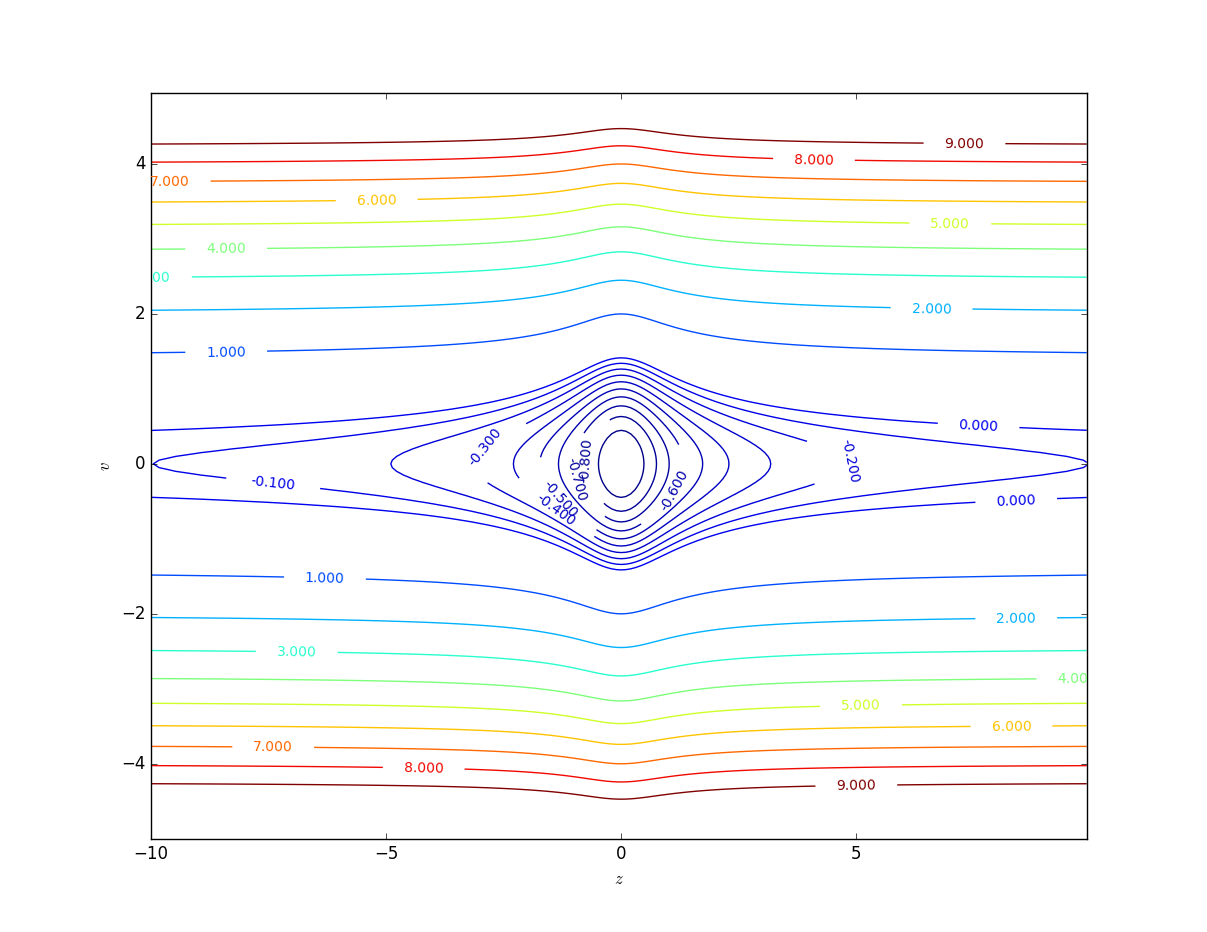
\includegraphics[scale=0.3]{figure_1.png}
\caption{Energy level for two equal mass primaries}\label{fig:energy}
\end{center}
\end{figure}

Now we will prove the second item of the theorem. We consider a $T_0$-periodic solution ($E<0$).  As a consequence of the symmetries of the equation we have that the curve $t\mapsto (z(t),v(t))$, for $0\leq t\leq T_0/4$, joins the points $(0,v_{E})$ and $(z_E,0)$. Then, taking account \eqref{eq:conser.energ} we have that
\begin{equation}
 \begin{split}
  \frac{T_0}{4}&=\frac{1}{\sqrt{2}}\int_0^{T_0/4}\left(E+\sum_{i=1}^n m_i (s_i^2+z^2)^{-\frac12}\right)^{-\frac12} z'(t) dt\\
  &=\frac{1}{\sqrt{2}}\int_0^{z_E}\left(\sum_{i=1}^n m_i \left((s_i^2+z^2)^{-\frac12}-(s_i^2+z_E^2)^{-\frac12}\right)\right)^{-\frac12}dz\\
  &=\frac{1}{\sqrt{2}}\int_0^{z_E} \left(z_E^2-z^2\right)^{-\frac12} f(z,z_E)dz\\
  &=\frac{1}{\sqrt{2}}\int_0^1 \left(1-u^2\right)^{-\frac12} f(z_Eu,z_E)du,
 \end{split}
\end{equation}
where \[f(z,z_E)=\left(\sum_{i=1}^n m_i \left\{(s_i^2+z^2)(s_i^2+z_E^2)\right\}^{-\frac12} \left\{(s_i^2+z^2)^{-\frac12}+(s_i^2+z_E^2)^{-\frac12} \right\}\right)^{-\frac12}.\]
We note that $f(z_Eu,z_E)$ is a increasing function with respect to $z_E$ for $u\in [0,1]$ fix. Additionaly
\begin{equation*}
 \lim\limits_{z_E \to 0}f(z_Eu,z_E)=\left(\sum_{i=1}^{n} \frac{m_i}{2s_i^3}\right)^{-\frac12} \quad \text{and}\quad  \lim\limits_{z_E \to \infty}f(z_Eu,z_E)=\infty.
\end{equation*}
Therefore, from the dominated convergence theorem and monotone convergence theorem we have that
\[\lim\limits_{z_E\to 0}T_0=2\pi\left(\sum_{i=1}^{n} \frac{m_i}{s_i^3}\right)^{-\frac12}\quad \text{and}\quad \lim\limits_{z_E\to \infty}T_0=\infty.\]
Finally,  since $T_0=T_0(z_E)$ is continuous and increasing respect to $z_E$ we conclude the afirmation in the item \ref{2}.



The item \ref{3} is consequence that $T^2=4\pi^2 \sum_{i=1}^{n}m_i|q_i|^2/U$   (see \cite[p. 109]{JaumeLlibre276}).
\end{proof}






Let us to show a second proof of item \ref{2} of Theorem \ref{thm:prin_ine}. For the sufficiency we  follow arguments of \cite{zhao2015nonplanar} and \cite{li2013characterization}, based on variational principles. For the necessity of condition \eqref{eq:ine_T0-per-cond} we use Sturm's comparison theorem.


\begin{proof}[Alternitave Proof Theorem \ref{thm:prin_ine} (\ref{2})]

First we prove that \eqref{eq:ine_T0-per-cond} is a necessary condition for the existence of a $T_0$-periodic solution. We assume that $z$ is a $T_0$-periodic solution of \eqref{eq:eq_new_red}.
Using Sturm's Comparison Theorem (see \cite{birkhoff1989ordinary}) with equations  $z''+q_1(z)z=0$, where $q_1(z)=\sum_{i=1}^{n} m_i \left(s_i^2 +z^2\right)^{-3/2}$, and $z''+\left(\sum_{i=1}^{n} m_i s_i^{-3}\right)z=0$ we deduce \eqref{eq:ine_T0-per-cond}.



Let $T_0>0$ satisfiying \eqref{eq:ine_T0-per-cond}. We consider the action integral
\[\mathcal{I}(z)=\int_0^{T_0}\frac12|z'|^2+\sum_{i=1}^n\frac{m_i}{\sqrt{s_i^2+z^2}}dt,\]
Then $T_0$-periodic solutions of \eqref{eq:eq_new_red} are critical points of $\mathcal{I}$ in the space $H^1(\mathbb{T},\rr)$, where $\mathbb{T}=\rr/T_0\mathbb{Z}$, of the functions  absolutely continuous, $T_0$-periodic with $z'\in L^2(\mathbb{T},\rr)$ (see \cite[Cor. 1.1]{Mawhin2010}). We prove the existence of critical points by means of the direct method of calculus of variations, i.e. we will prove that $\mathcal{I}$ has minimum.  The functional $\mathcal{I}$ is not coercive in $H^1(\mathbb{T},\rr)$,  this deficiency is drawn with symmetry techniques (see \cite{David-2004}). The group $\mathbb{Z}_2$ acts on $H^1(\mathbb{T},\rr)$ according to the following assignments $(\bar{0}\cdot z)(t)=z(t)$ and $(\bar{1}\cdot z)(t)=-z(t+\frac{T_0}{2})$. The functional $\mathcal{I}$ is $\mathbb{Z}_2$-invariant, i.e. $\mathcal{I}(g\cdot z)=\mathcal{I}(z)$. We define the space of all $\mathbb{Z}_2$-symmetric (this simmetry is called the italian simmetry) funcions \[\Lambda(\mathbb{T},\mathbb{R}):
=\left\{ z\in H^1(\mathbb{T},\rr) | \forall g\in \mathbb{Z}_2 : z=g\cdot z \right\}.\]
The funciontal $\mathcal{I}$ restricted to $\Lambda$  is coercive. This fact follows from an obvious adaptation of proposition 4.1 of \cite{David-2004}. We note that $F(z):=\sum_{i=1}^nm_i(s_i^2+z^2)^{-\frac{1}{2}}$ satisfies the condition $(A)$ in \cite[p. 12]{Mawhin2010}, then $\mathcal{I}$  is continuously differentiable and weakly lower semicontinuous on $H^1(\mathbb{T},\rr)$ (see \cite[p. 13]{Mawhin2010}). Therefore $\mathcal{I}$ has a minimum $z_0$ in $\Lambda(\mathbb{T},\mathbb{R})$. Then by the Palais' principle symmetric criticality,  $z_0$ is a critical point of $\mathcal{I}$ in $H^1(\mathbb{T},\rr)$ (see \cite{David-2004} and \cite{RichardPalais274}).

We use the second variation $\delta^2 \mathcal{I}$ in order to show  that $z_0\nequiv 0$. It is well known (see \cite[Th. 1.3.1]{jost1998calculus}) that if $z_0$ is a minimum of $\mathcal{I}$ on $H^1(\mathbb{T},\rr)$  then $\delta^2 \mathcal{I} (z_0,\varphi)\geq 0$ for all $\varphi\in H^1(\mathbb{T},\rr)$. In our case
\[\delta^2\mathcal{I}(0,\varphi)=\int_0^{T_0} |\varphi'|^2-\sum_{i=1}^{n}\frac{m_i}{r_i^3}\varphi^2 dt,\]
(see \cite[Eq. 1.3.6]{jost1998calculus}). In particular for $\varphi(t)=\sin (2\pi t/T_0)$ it follows from \eqref{eq:ine_T0-per-cond}  that
\begin{equation}\label{eq:form.delta2}
 \delta^2 \mathcal{I} (0,\varphi)=\left( \frac{4\pi^2}{T_0^2}-\sum_{i=1}^{n}\frac{m_i}{r_i^3} \right)\frac{T_0}{2}<0.
\end{equation}
It is sufficient  to guarantee that $z_0\equiv 0$ is not a minimum.
\end{proof}

\begin{comentario}
We note that this second proof of Theorem \ref{thm:prin_ine} (\ref{2}), unlike the first one, does not guarantee that $T_0$ is the minimum period for $z_0$. It could happen that $z_0$ had period $T_0/m$, with natural $m\in\mathbb{N}$. Because of Italian symmetry this $m$ should be odd.
\end{comentario}


\begin{proof}[Proof Corollary \ref{cor:nleq472}]
In this case $s_1=s_2=\cdots=s_n=:r$ and $m_1=m_2=\cdots=m_n=:m$. Then, from the law of cosines we obtain
\[
 \sum_{i<j}\frac{m_im_j}{r_{ij}}=\frac{nm^2}{4r}\sum_{j=1}^{n-1}\frac{1}{\sin\left(\frac{j\pi}{n}\right)}.
\]
Therefore the condition \eqref{eq:ine_prin} is equivalent to

\begin{equation}\label{eq:ine_prin_LShShao}
  \frac1n\sum_{j=1}^{n-1}\frac{1}{\sin\left(\frac{j\pi}{n}\right)}<4.
\end{equation}

This inequality was also derived by Li, J. et al. in \cite{li2013characterization}. In this paper the authors noted (performing calculations with computer) that inequality \eqref{eq:ine_prin_LShShao} holds true for $2\leq n\leq 472$. Let us prove that any other $n$ satisfies \eqref{eq:ine_prin_LShShao}.

We suppose first that $n=2k$ is even. We note that

$$ \sum_{j=1}^{2k-1}\frac{1}{\sin\left(\frac{j\pi}{2k}\right)}= \sum_{j=1}^{k-1}\frac{1}{\sin\left(\frac{j\pi}{2k}\right)}+1 +\sum_{j=k+1}^{2k-1}\frac{1}{\sin\left(\frac{j\pi}{2k}\right)},$$
and
$$ \sin\left(\frac{(k-j)\pi}{2k}\right)=\sin\left(\frac{(k+j)\pi}{2k}\right)=\cos\left(\frac{j\pi}{2k}\right).$$
Therefore, $n$ does not satisfies \eqref{eq:ine_prin_LShShao} when

\begin{equation}\label{eq:ine_prin_LShShao.2k}
 \frac{1}{k}\sum_{j=1}^{k-1}\frac{1}{\cos\left(\frac{j\pi}{2k}\right)}+\frac{1}{2k}\geq 4.
\end{equation}
Since $1/\cos(x)$ is an increasing function on $[0,\pi/2)$ then

$$ f\left(\frac{\pi}{2 }\frac{(k-1)}{k}  \right)=
\int_0^{\frac{\pi}{2 }\frac{(k-1)}{k} }\frac{dx}{\cos x}
\leq \frac{\pi}{2k}\sum_{j=1}^{k-1}\frac{1}{\cos\left(\frac{j\pi}{2k}\right)}, $$
where
$$f(x)=\log\sqrt{\frac{1+\sin(x)}{1-\sin(x)}}.$$
Hence, the following inequality implies \eqref{eq:ine_prin_LShShao.2k}

$$4\leq \frac{2}{\pi}f\left(\frac{\pi}{2 }\frac{(k-1)}{k}  \right) +\frac{1}{2k}:=g(k)$$
An elementary analysis shows that $g(k)$ is an increasing function with respect to $k$, and $g(420)\approx 4.00032$. Consequently we have proved that if $n$ is even and satisfies \eqref{eq:ine_prin_LShShao} then $n\leq 840$.

Reasoning in a similar way, we obtain an analogous result for the case $n$ odd.

In this way we have proved that the inequality \eqref{eq:ine_prin_LShShao} is false for all $n$ greater than a certain $n_0$.

The validity of the inequality \eqref{eq:ine_prin_LShShao}, for $n\leq n_0$, is easily established using computer. This gives the result that the inequality holds for all $n \leq 472$.
\end{proof}

\begin{proof}[Proof Theorem \ref{thm:CC.3.4.satis.cond.adm}]

Let's start by analyzing the central configuration CCr. We can suppose without loss of generality that $ q_1 = -q_3 = (0, y) $ for $ y> 0 $, $ q_2 = -q_4 = (1,0) $, $ m_1 = m_3 = M $, $ m_2 = m_4 = m $ and $ M> m $. Then, necessarily $ y <1 $ (see \cite{perez2007convex}). For this CC  the condition \eqref{eq:ine_prin} becomes
\[\frac{M^2}{2y}+\frac{4Mm}{\sqrt{1+y^2}}+\frac{m^2}{2}<\left(\frac{2M}{y^3}+2m\right) \left(2My^2+2m\right).\]
As $M^2/(2y)<4M^2/y$, $m^2/2<4m^2$ and $4Mm/\sqrt{1+y^2}<4Mm/y^3$ (since $y<1$), we have that the inequality holds.

 Now consider the central configuration CCl.  Remark first that some of the following calculations were computed using a symbolic mathematics  software.  We can suppose without loss of generality that $q_1=-q_3=1$, $q_2=-q_4=x$ with $0<x<1$, and $m_1=m_3=\mu$, $m_2=m_4=1-\mu$, with $0<\mu<1$.  Then the inequality \eqref{eq:ine_prin} becomes
\[\frac{2\mu(1-\mu)}{1-x} +\frac{2\mu(1-\mu)}{1+x}+\frac{\mu^2}{2}+\frac{(1-\mu)^2}{2x}<4\mu^2+4\mu(1-\mu)x^2+\frac{4\mu(1-\mu)}{x^3}+\frac{4(1-\mu)^2}{x}.\]
As $ \frac{\mu ^ 2}{2} <4 \mu^2$ and $ \frac{(1-\mu)^2}{2x}< \frac{4(1-\mu)^2}{x} $ (without taking into account the term $4\mu(1- \mu)x^2$) we just have to show that
\[\frac{2\mu(1-\mu)}{1-x} +\frac{2\mu(1-\mu)}{1+x}<\frac{4\mu(1-\mu)}{x^3},\]
and this is equivalent to see that
\begin{equation}\label{eq:ineq.4.cuerpos.alinea}
\frac{x^3}{1-x^2}<1.
\end{equation}
The values of $x$ involved in the above inequality are such that the configuration for the vector mass $(\mu,1-\mu,1-\mu,\mu)$ is central, by Moulton \cite{moulton1910straight}, fixed a mass $\mu$ there is only one value $x$ satisfiying this condition. So, we can define $x(\mu)$ as such value of $x$. If we can see that the funcion $x(\mu)$ is a decreasing function, then we have that
$\frac{x(\mu)^3}{1-x(\mu)^2}\leq \lim\limits_{\mu\to 0}\frac{x(\mu)^3}{1-x(\mu)^2}.$
If also we demonstrate that 
\begin{equation}\label{eq:ineq.4.cuerpos.lim0}
\lim\limits_{\mu\to 0}\frac{x(\mu)^3}{1-x(\mu)^2}<1
\end{equation} 
we have tested \eqref {eq:ineq.4.cuerpos.alinea}. 

Let's first prove that $x(\mu)$ is a decreasing function. The relationship between $\mu$ and $x$ follows from the fact that the bodies are in a central configuration. Therefore the equation 
\[\frac{\mu}{4} - \frac{\mu}{x \left(x + 1\right)^{2}} + \frac{\mu}{x \left(- x + 1\right)^{2}} + \frac{- \mu + 1}{\left(x + 1\right)^{2}} + \frac{- \mu + 1}{\left(- x + 1\right)^{2}} - \frac{1}{x^{3}} \left(- \frac{\mu}{4} + \frac{1}{4}\right) = 0\]
 must be satisfied, simplifying this expression we have 
 \[\frac{p(\mu,x)}{q(\mu,x)}  = 0,\]
 where $p(\mu,x)=\mu x^{7} - 10 \mu x^{5} + \mu x^{4} + 9 \mu x^{3} - 2 \mu x^{2} + \mu + 8 x^{5} - x^{4} + 8 x^{3} + 2 x^{2} - 1$ and $q(\mu,x)=4 x^{3} \left(x^{4} - 2 x^{2} + 1\right)$. So the relationship between $\mu$ and $x$ is given that $p(\mu,x)=0$. We can derive implicitly the last equation an we obtain 
 \[\frac{dx}{d\mu}=\frac{Np(x)}{Dp(x,\mu)},\]
 where $Np(x)=- \left(x - 1\right) \left(x + 1\right) \left(x^{5} - 9 x^{3} + x^{2} - 1\right)$ and  $Dp(x,\mu)=\mu x^2\left(7 x^{4} - 10 x^{2} + 51 \right) +\left(1- \mu \right) \left( 40 x^{4} + 20 x^{3}  + 4 x \right)$. The denominator $Dp(x,\mu)$ is clearly positive for $0<x<1$ and $0<\mu<1$. To prove that the numerator $Np(x)$ is negative let's see that the polynomial $x^{5} - 9 x^{3} + x^{2} - 1$ is negative for all $0 <x <1$. In fact, calculating their real roots with a software we have that these are  $-3.0483999$, $-0,449322$ and $2,94956549$, then it is easy to see that $x^{5} - 9 x^{3} + x^{2} - 1$ is negative in the interval $(0,1)$, hence $Np(x)<0$ for $0<x<1$. This implies that $\frac{dx}{d\mu}$ is negative for all $0<x<1$ and $0<\mu<1$.

Let's see now that \eqref{eq:ineq.4.cuerpos.lim0} holds. Since $x(\mu)$ is a continuous function we need to prove $\frac{x(0)^3}{1-x(0)^2}<1$. For simplicity we will write $x$ instead of $x(0)$. This value $x$ is such that $p(0,x)=8 x^{5} - x^{4} + 8 x^{3} + 2 x^{2} - 1 = 0$,  then  $8 x^{5} + 8 x^{3} = \left(x^{2} - 1\right)^{2}$, and this implies that $8 x^{5} + 8 x^{3}<1$, hence $x^3<1/(8(x^2+1))<1/8$, $x^2<(1/8)^{\frac23}$ and
\[\frac{x^3}{1-x^2}<\frac{1/8}{1-1/8^{\frac23}}=\frac16<1,\]
as we wanted to prove.
\end{proof}







\section*{Acknowledgments}



\bibliographystyle{plainurl}
 %\bibliographystyle{apalike-url}
 \bibliography{mecanica_celeste}


\end{document}
